\begin{figure}[H]
\centering
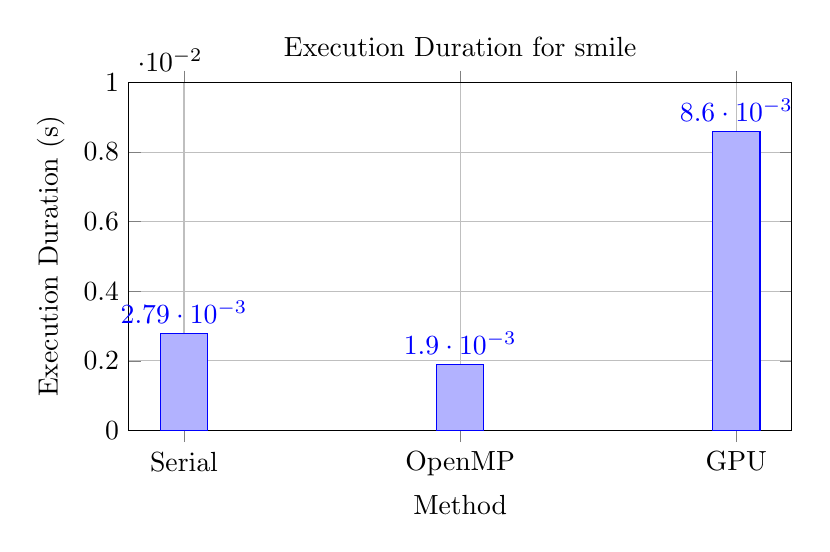
\begin{tikzpicture}
    \begin{axis}[
        ybar,
        bar width=.6cm,
        width=10cm,
        height=6cm,
        ylabel={Execution Duration (s)},
        xlabel={Method},
        symbolic x coords={Serial, OpenMP, GPU},
        xtick=data,
        nodes near coords,
        ymin=0, ymax=0.01,
        grid=major,
        title={Execution Duration for smile}
    ]
        \addplot coordinates {(Serial,0.00278600) (OpenMP,0.00190175) (GPU,0.00859648)};
    \end{axis}
\end{tikzpicture}
\caption{Comparison of execution duration for the dataset Circle: N1000 with different implementation methods. Experiments are conducted on an Intel i9-13980HX consumer CPU and NVIDIA RTX4070 consumer GPU with 512 threads per thread block}\label{fig:smile}
\end{figure}
